\title{Study Guide for Midterm 1}
\author{Dr. Jordan Hanson - Whittier College Dept. of Physics and Astronomy}
\date{\today}
\documentclass[10pt]{article}
\usepackage[a4paper, total={18cm, 27cm}]{geometry}
\usepackage{outlines}
\usepackage{graphicx}
\begin{document}
\maketitle

\textbf{Instructions:} Work each problem \textit{before} checking your answer with the key (to follow on Moodle). \\ \vspace{0.25cm}

\section{Memory Bank}

\begin{enumerate}
\item $m = \rho V$ ... Mass is the density times the volume
\item $V = \frac{4}{3}\pi r^3$ ... The volume of a sphere
\item $\vec{F} = k \frac{q_1 q_2}{r^2}\hat{r}$ ... Coulomb Force
\item $k = 9 \times 10^{9}$ N C$^{-2}$ m$^{2}$ ... Remember $k = 1/(4\pi \epsilon_0)$.
\item $q_e = 1.6 \times 10^{-19}$ C ... Charge of an electron/proton
\item Atomic mass: the number of grams per mole of a substance
\item $N_A = 6.03 \times 10^{23}$ ... Avagadro's number
\item $\vec{F} = q \vec{E}$ ... Electric field and charge
\item $\vec{E}(z) = \frac{\sigma}{\epsilon_0}\hat{z}$ ... Electric field of two oppositely charge planes each with charge density $\sigma$
\item $\epsilon_0 \approx 8.85 \times 10^{-12}$ F/m
\item $U = q\Delta V$ ... Potential energy and voltage
\item 1 eV: an electron-Volt is the amount of energy one electron gains through 1 V.
\item $V(r) = k\frac{q}{r}$ ... Voltage of a point charge
\item $\vec{E} = -\frac{\Delta V}{\Delta x}$ ... E-field is the slope or change in voltage with respect to distance
\item $V(x) = -E x + V_0$ ... Voltage is linear between two charge planes
\item $Q = CV$ ... Definition of capacitance
\item $C = \frac{\epsilon_0 A}{d}$ ... Capacitance of a parallel plate capacitor
\item $C_{tot}^{-1} = C_1^{-1} + C_2^{-2}$ ... Adding two capacitors \textit{in series.}
\item $C_{tot} = C_1 + C_2$ ... Adding two capacitors \textit{in parallel.}
\end{enumerate}

\clearpage

\section{Electric Charge and Electric Fields}

\begin{enumerate}
\item (a) A certain lightning bolt moves 40.0 C of charge.  To how many electrons does this correspond? (b) Suppose a speck of dust in an oil drop experiment\footnote{A great paper topic, by the way: the Millikan oil drop experiment.} has  $10^{12}$  protons in it and has a net charge of -5.00 nC (a very large charge for a small speck). How many electrons does it have?\\ \vspace{1cm}
\item (a) Two charges exert $F_{\rm C} = 5.00$ N of force on each other. What will $F_{\rm C}$ be if the distance between them triples? (b) If one charge is $1$ nC, and the other is $2$ nC, what is the distance between them if $F_{\rm C} = 5.00$ N? \\ \vspace{1cm}
\item 
\begin{figure}
\centering
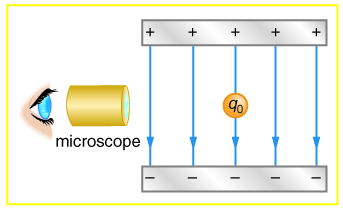
\includegraphics[width=0.3\textwidth]{mill.jpeg}
\caption{\label{fig:mill} The classic Millikan oil drop experiment was a measurement of the charge of an electron.}
\end{figure}
The classic Millikan oil drop experiment was the first to measure accurately the electron charge. Oil drops were suspended against the gravitational force by a vertical electric field. (See Fig. \ref{fig:mill}.) The drops have radius $1.0 \mu$m, and a density of 920 kg/m$^3$. (a) Find the weight of the drop. (b) If the drop has a single excess electron, find the electric field strength needed to balance its weight. \\ \vspace{1.75cm}
\item Suppose two positive, identical charges are located a distance $d$ apart. (a) Sketch the electric field below.  (b) Sketch the electric field if instead one of the charges is negative. \\ \vspace{2.5cm}
\item Suppose three electrons are arranged in an equilateral triangle 0.1 nm on a side (see Fig. \ref{fig:tri}).  (a) What is the electric field \textbf{vector} at the location of the top charge? (b) Where is the electric field zero?
\begin{figure}[ht]
\centering
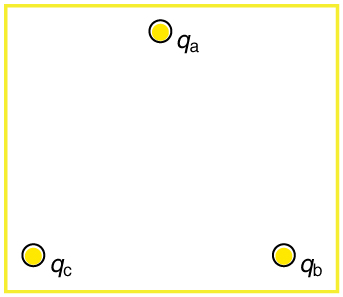
\includegraphics[width=0.25\textwidth]{tri.jpeg}
\caption{\label{fig:tri} An equilateral triangle, $0.1$ nm on a side (internal angles are 60 degrees).}
\end{figure}
\end{enumerate}

\section{Potential Energy and Voltage}

\begin{enumerate}
\item What is the electric field across an 10.00 nm thick membrane if (a) the voltage across it is 50 mV? You may assume a uniform electric field. (b) Suppose this cell membrane is part of a nerve cell.  How much energy would an electron gain if dropped through the 50 mV voltage and accelerated across the cell freely?  Express your anser in electron-Volts (eV). \\ \vspace{2cm}
\item \textbf{Think back to the PhET simulations of parallel lines of charge.}  Suppose a parallel plate capacitor is formed from a positive plate and a negative plate of charge.  The plates' areas $A$ are the same, and the plates' charges ($\pm Q$), and charge densities ($\pm Q/A = \pm \sigma$) are the same as well. (a) Write the expression for the electric field between the plates. (b) Suppose $Q = 1$ nC, and $A = 10$ mm$^2$.  What is the value of the electric field between the plates?  (c) Suppose 0 volts corresponds to the location of the negative plate.  Draw the voltage as a function of distance between the plates.  (d) What is the voltage near the positive plate, if the plates are are separated by a distance $d = 1$ mm? \\ \vspace{2cm}
\end{enumerate}

\section{Capacitors}

\begin{enumerate}
\item What is the capacitance of the capacitor in the previous problem? \\ \vspace{1cm}
\item (a) Consider the same capacitor again, and suppose a second identical capacitor is connected \textit{in parallel} with it.  What is the total capacitance? (b) How much charge would the pair of capacitors store if the voltage across them was 5 volts? \\ \vspace{1.5cm}
\item How much energy in Joules would this charge have if it was all put to work?
\end{enumerate}

\end{document}